%TODO(jpdarago): Hacer grafico con Turbo Boost

Asi como ya exist\'ia una base de c\'odigo original de CUDA, el
trabajo sobre CPU tambi\'en se realiz\'o sobre el c\'odigo original
existente. El mismo fue dise\~nado de manera uniprocesador, y teniendo
en mente un conjunto de instrucciones SIMD anterior a AVX, donde el tama\~no
de los registros de procesador era de 128 bits.

Con el prop\'osito de adaptar el c\'odigo para procesadores
paralelos y vectoriales como lo son los de la gama Xeon y Xeon Phi de
Intel, se busc\'o vectorizar y paralelizar el c\'odigo tanto como fuese
posible. En particular, se prioriz\'o lograr una gran escalabilidad en
n\'umero de procesadores, especialmente en las pruebas realizadas en el
Xeon.

De acuerdo a la bibliografia~\cite{Jeffers}, es necesario lograr que
el c\'odigo este no solamente bien vectorizado sino que escale con la
cantidad de procesadores para poder hacer uso de las prestaciones del
coprocesador Xeon Phi. Por lo tanto, las pruebas iniciales se concentraron
en lograr buena escalabilidad y vectorizac\'on en CPU \'unicamente.

Puesto que muchas decisiones arquitecturales del c\'odigo se realizaron en
base a experimentos con prototipos representativos de las diversas operaciones,
incluiremos algunos detalles del dispositivo utilizado para las pruebas.

La computadora utilizada para las pruebas fue un servidor \textit{dual-socket}
con 2 Intel Xeon CPU E5-2620 v2, con 6 cores cada uno. Los
procesadores corren a una frecuencia de clock de 2.10 GHz, y soportan el set
de instrucciones x86-64 con AVX 1.
Cada procesador cuenta con 64 Kb de cach\'e L1, 2 Mb de cach\'e L2 para cada par de cores, y
15 Mb de cach\'e L3 compartida.
El mismo contaba con 32 GB de memoria RAM DDR3 a 4 canales de memoria, dando
una transferencia te\'orica m\'axima de 42.6 GB/s, con ciclo de clock a 1.3 GHz.

La familia de procesadores Xeon cuenta con tecnolog\'ia Turbo Boost. La misma
incluye una funcionalidad en el chip que ajusta din\'amicamente la frecuencia
de los procesadores de acuerdo a la temperatura y potencia empleadas. Esto, si
bien a \textit{a priori} es algo \'util ya que mejora la performance de los
programas, dificulta el an\'alisis de escalabilidad ya que al utilizar m\'as
procesadores, aumenta el consumo energ\'etico y temperatura y por tanto la
frecuencia de los procesadores disminuye. Para evitar este efecto en nuestro
an\'alisis se deshabilito Turbo Boost al realizar las pruebas.

Asimismo, originalmente los procesadores Intel Xeon cuentan con Hyperthreading,
permitiendo 2 procesadores l\'ogicos sobre uno f\'isico, dando un total de 24 procesadores.
Sin embargo, los dos hilos de ejecuci\'on (\textit{hyperthreads}) en un mismo
procesador comparten unidades b\'asicas como las ALU. Al no ser totalmente
independientes, esto tambi\'en dificulta el an\'alisis. Para no tomar esto en
cuenta se trabajo con Hyperthreading deshabilitado.

Las pruebas tambi\'en se ajustaron en base al coprocesador Xeon Phi que estaba
conectado al Xeon como host. El modelo de coprocesador usado contaba con 61
cores y 8 Gb de memoria RAM, los valores est\'andar para la l\'inea actual de
Xeon Phi.

La secci\'on de c\'odigo trabajada corresponde a la parte del procesamiento
de LIO optimizada mediante CUDA. Esta parte del c\'odigo estaba ya implementada
en C++, utilizando librer\'ias de Intel ICC para vectorizaci\'on. Al momento
de empezar la optimizaci\'on, las subrutinas asociadas insum\'ian la mayor
cantidad de tiempo. La optimizaci\'on de otros c\'alculos por fuera de la
energ\'ia de intercambio y correlaci\'on quedan fuera del \textit{scope} de este
trabajo.

\subsection{Caso de estudio}

Para las pruebas de esta secci\'on se utiliz\'o el grupo hemo, el
cual es un caso muy utilizado dentro de la literatura. Detalles sobre este
sistema y otros utilizados se encuentran en un ap\'endice de este trabajo.

El par\'ametro de tama\~no de los cubos utilizado es 3, el valor m\'as
apropiado al momento de iniciar el trabajo sobre la implementaci\'on para CPU.

El an\'alisis realizado corresponde a la implementaci\'on con precisi\'on simple,
aunque los mismos aplican de igual manera para precisi\'on doble (no se necesita
m\'as que recompilar el c\'odigo para utilizar precisi\'on doble). Experimentos
presentados m\'as adelante detallan como se modifica el tiempo de ejecuci\'on al
usar precisi\'on doble.

% TODO(jpdarago): Agregar datos de hemoglobina en el apendice

\subsection{Estructura original del c\'odigo}

Un esquema de alto nivel del computo m\'as intensivo realizado por el m\'odulo
XC se encuentra en la figura~\ref{algo:lio-iteration}. Este c\'odigo corresponde
a una iteraci\'on del c\'alculo de la matriz de Kohn-Sham y se compone de tres
partes, el c\'alculo de las matrices relacionadas con las funciones, calcular las
densidad electr\'onica, su gradiente y hessianos para cada punto, y utilizarlos
para obtener la energ\'ia de intercambio y correlaci\'on, la contribuci\'on a
la matriz de Kohn Sham y, al lograr la convergencia, a la matriz de fuerzas.

\begin{algorithm}[H]
        \caption{Pseudoc\'odigo de la iteraci\'on original de LIO}
        \label{algo:lio-iteration}
        \begin{algorithmic}
            \Function{solve}{$PG : PointGroup$}
              \State Leer la matriz de coeficientes inicial.
              \State Calcular funciones, su gradiente y hessiano.
              \ForAll{$p \in puntos(PG)$}
                  \ForAll{$i \in functions(PG, p)$}
                       \State Calcular la contribuci\'on a la densidad, $dens$
                       \State Calcular la contribuci\'on al gradiente, $grad$
                       \State Calcular la contribuci\'on a los hessianos, $hess$
                  \EndFor
                  \State Calcular potencial usando $dens$ y $grad$.
                  \State Calcular contribuci\'on $FR_p$ a KS y Fuerzas usando $dens$, $grad$ y $hess$.
                  \State Calcular energ\'ia resultado $energy$ con potencial y el peso del punto $p$.
              \EndFor
              \State Calcular fuerzas usando los factores $FR$ y los n\'ucleos de los \'atomos.
              \State Sumar la contribuci\'on de cada punto a la matriz de Kohn-Sham general.
            \EndFunction
        \end{algorithmic}
\end{algorithm}

Un aspecto importante a se\~nalar es la representaci\'on de las matrices en el
programa.

Las matrices del gradiente y hessiano tienen como elementos vectores $\mathbb{R}^3$, y
la matriz de valores de funciones es una matriz de escalares. Las operaciones entre
vectores y vectores y entre vectores y escalares tienen la sem\'antica esperable de \'algebra
lineal. El producto entre dos vectores en el c\'odigo debe ser interpretado como producto
componente a componente, no como producto escalar o vectorial.

La implementaci\'on de las operaciones entre vectores merece particular atenci\'on.
Para aprovechar el set de instrucciones SSE 4, la ultima versi\'on disponible al
momento de realizar la implementaci\'on, el tipo de datos para un vector de 3
componentes (\texttt{cvector3}) se adapt\'o para corresponderse a un
registro de SSE 4. Dado que el ancho de estos registros es de 128 bits, los mismos
permiten realizar c\'alculos de a 4 elementos de punto flotante a la vez. Al ser 3, uno de los
elementos del registro SSE no se utiliza (fijandole el valor en 0).~\cite{Nitsche2014}.
Es tarea del compilador luego traducir las operaciones usuales a instrucciones
vectoriales.

La representaci\'on de un vector $\mathbb{R}^3$ de esta manera, si bien da
un \textit{speedup} significativo, no es portable ni escalable a otras extensiones
SIMD. Al incrementar el ancho de registro un n\'umero mayor de los campos deben ser ignorados, malgastando cada
vez m\'as espacio \'util. Asimismo, se desperdician oportunidades por parte del compilador
para optimizar mejor haciendo uso de todos los registros y operaciones que dispone
la arquitectura sobre la cual se esta compilando, ya que se le dice expl\'icitamente
que operaciones tiene que hacer y como.

Profiling del tipo de iteraci\'on m\'as com\'un de la implementaci\'on inicial se encuentra en la figura~\ref{fig:initial-profiling}.
Como puede verse, el gran dominante son los c\'alculos correspondientes a la densidad electr\'onica,
que incluyen los dos primeros ciclos del pseudoc\'odigo de
la figura~\ref{algo:lio-iteration}. Tambi\'en vemos la importancia de
la actualizaci\'on de la matriz de Kohn-Sham y el c\'alculo de las matrices de
funciones gradiente y hessiano, que no son despreciables pero son peque\~nas en
comparaci\'on. Omitimos el c\'alculo de fuerzas pues este se realiza solamente
en la \'ultima iteraci\'on.

\begin{figure}[htbp]
   \centering
   \includegraphics[width=\plotwidth]{plots/cpu/initial-iteration-parts-hemo.png}
   \caption{Divisi\'on de los tiempos de iteraci\'on para la hemoglobina en la versi\'on
   original en CPU}
   \label{fig:initial-profiling}
\end{figure}

\subsection{Cambios en la vectorizaci\'on}

Dado el peso los c\'omputos internos para la densidad electr\'onica y la energ\'ia
de intercambio y correlaci\'on, empezamos por eliminar la dependencia expl\'icita
con SIMD, eliminando la herencia de esta clase con los tipos de datos de SSE.

Esto deleg\'o al compilador la tarea de vectorizar el c\'odigo apropiadamente. En consecuencia
se produjo al principio una degradaci\'on importante de performance, dado que las operaciones
de suma, multiplicaci\'on, etc. involucrando vectores ya no eran vectorizadas por defecto, y
las mismas son parte muy importante del algoritmo de c\'alculo de la energ\'ia.

Esto se resolvi\'o con una reorganizaci\'on en memoria de las matrices. La observaci\'on clave
para esto es que las operaciones se realizan de a una componente por vez. En particular,
el ciclo m\'as intensivo de c\'omputo (el interior de la iteraci\'on, detallado en el pseudoc\'odigo
de la figura~\ref{algo:lio-inner-cicle}) puede dividirse
en cada componente para convertirse en 10 operaciones de suma sobre un producto de
dos vectores.

\begin{algorithm}[H]
        \caption{Pseudoc\'odigo del ciclo principal del c\'alculo de la energ\'ia de intercambio y correlaci\'on}
        \label{algo:lio-inner-cicle}
        \begin{algorithmic}
            \Function{solve}{$PG : PointGroup$}
              \ForAll{$p \in puntos(PG)$}
                  \ForAll{$i \in functions(PG, p)$}
                     \State $dens \gets \Sigma_{j = 0}^{i} MC_{i,j} \cdot F_{p,j}$
                     \State $grad \gets \Sigma_{j = 0}^{i} MC_{i,j} \cdot F_{p,j}$
                     \State $hess_1 \gets \Sigma_{j = 0}^{i} MC_{i,j} \cdot H_{2p,j}$
                     \State $hess_2 \gets \Sigma_{j = 0}^{i} MC_{i,j} \cdot H_{2p+1,j}$
                  \EndFor
                  \State Calcular la densidad en el punto usando $dens$,$grad$,$hess_1$ y $hess_2$
              \EndFor
            \EndFunction
        \end{algorithmic}
\end{algorithm}

Una heur\'istica de optimizaci\'on para estos casos es convertir los arreglos de
estructuras (como por ejemplo las matrices de gradiente $G$ y de hessiano $H$, que
son matrices densas de estructuras de tres valores) en estructuras de arreglos.
En este caso esto implica partir las matrices en 3 matrices (una para cada
componente), sino tambi\'en dividir el hessiano en sus componentes pares e impares.
De esta manera, cada componente es un valor escalar y los ciclos pueden reescribirse
para utilizar operaciones de punto flotante usuales sobre cada elemento.

Un esquema sencillo para visualizar la proyecci\'on realizada se muestra en
la figura~\ref{fig:matrix-split-img}. La clave es observar que ahora todos los
elementos de una misma componente est\'an consecutivos en memoria, con lo cual
pueden ser le\'idos y procesados de a tantos a la vez como se disponga mediante
registros SIMD. Anteriormente se pod\'ia procesar de a menos valores por
componente a la vez. Adem\'as, el c\'omputo puede aprovechar operaciones como
por ejemplo FMA (\textit{Fused Multiply Add}) que explicamos en secciones
anteriores.

\begin{figure}[htbp]
   \centering
   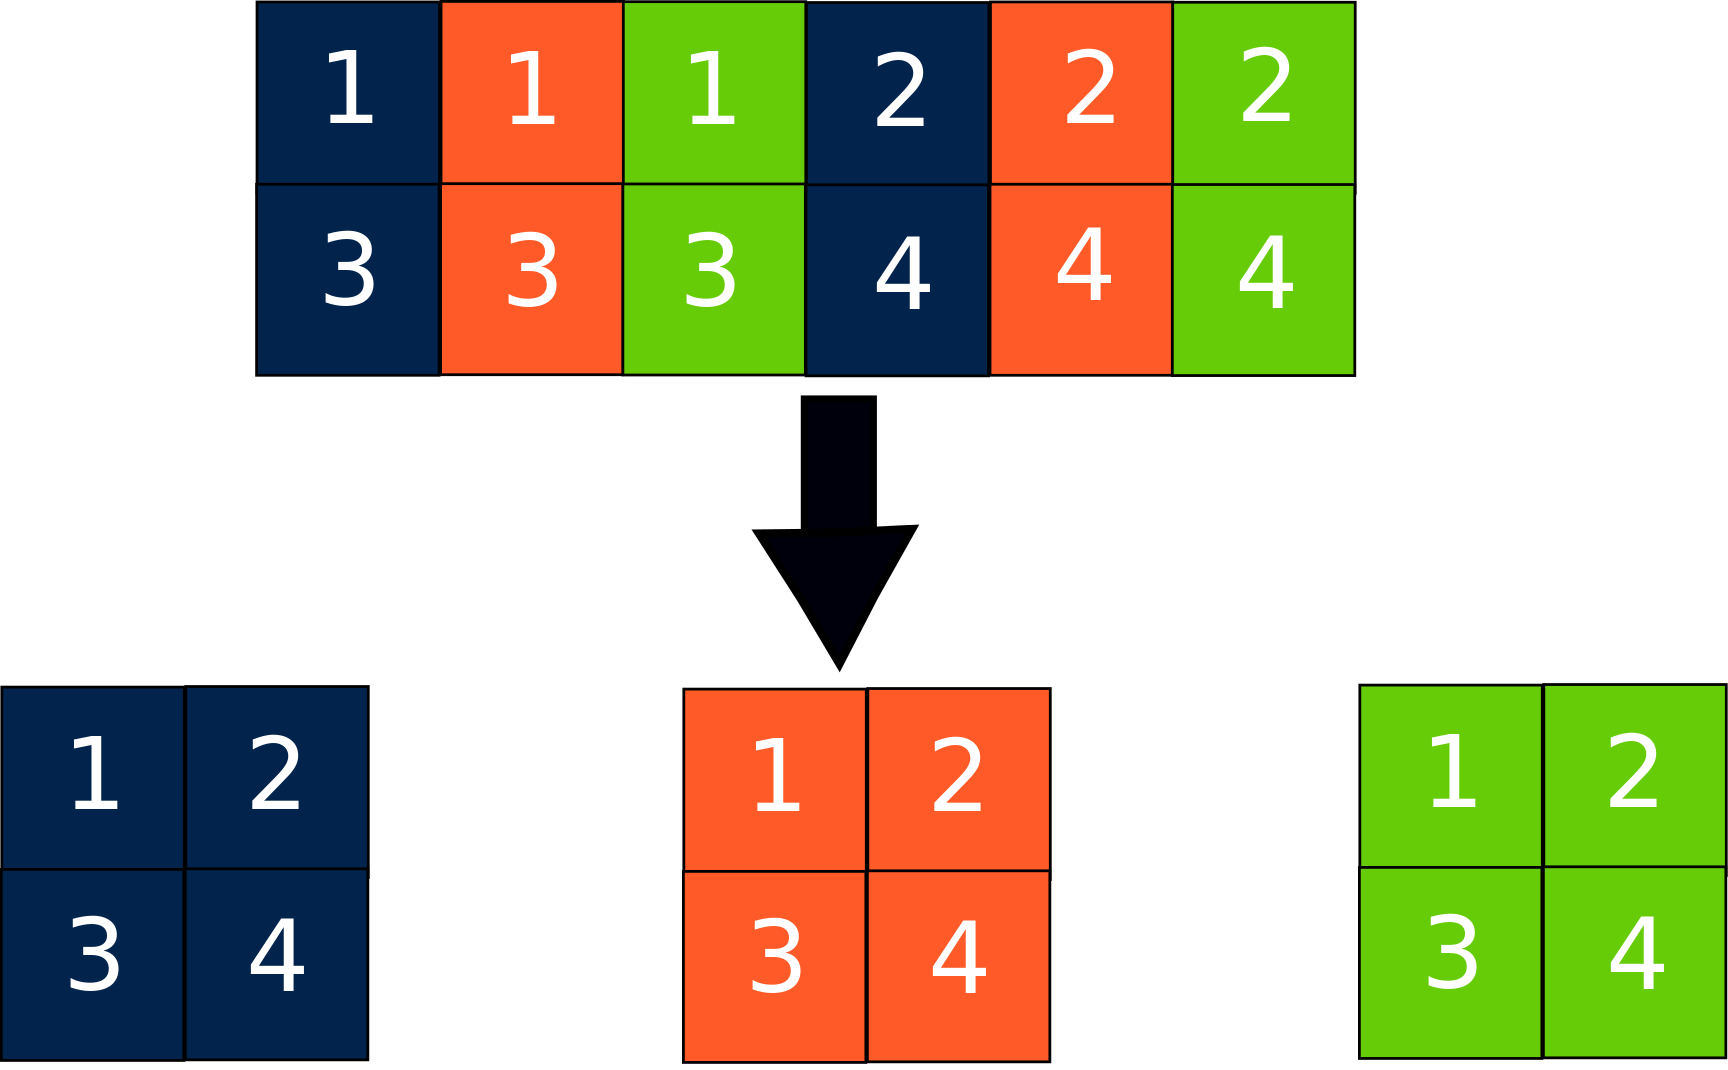
\includegraphics[width=\plotwidth]{images/matrix-split-img.png}
   \caption{Esquema de la proyecci\'on por componente realizada.}
   \label{fig:matrix-split-img}
\end{figure}

En el caso del hessiano de las funciones, el mismo tiene 6 componentes en vez
de 3, resultando entonces en 6 matrices separadas pero que funcionan de manera
an\'aloga a la matriz del gradiente.

Debido a la complejidad de los c\'alculos, y tratando de evitar introducir
errores sutiles, decidimos que al calcular las matrices de funciones, las
mismas se hicieran utilizando el c\'odigo  anterior pero con las versiones de
vectores sin SIMD, y luego proyectar las componentes a matrices en un \'ultimo
paso. Esto introduce un \textit{overhead} en los c\'omputos de funciones no
despreciable, pero veremos que este se puede palear con otras t\'ecnicas.

La figura~\ref{fig:lio-post-partir-mats} muestra los resultados de realizar esta
optimizaci\'on en el caso de prueba de hemoglobina en la computadora de prueba.
Como puede verse, la optimizaci\'on es muy significativa, incluso considerando
que incrementa el tiempo de c\'alculo de funciones (que todav\'ia se realiza en
todas las iteraciones) a\'un as\'i logra una aceleraci\'on sobre la versi\'on
original.

\begin{figure}[htbp]
   \centering
   \includegraphics[width=\plotwidth]{plots/cpu/post-split-matrices.png}
   \caption{Tiempo en segundos para la iteraci\'on de XC para el caso de la
   mol\'ecula de hemoglobina, antes y despu\'es de proyectar las componentes
   de las matrices.}
   \label{fig:lio-post-partir-mats}
\end{figure}

\subsection{Almacenamiento de las matrices}

Una mejora considerable surge tambi\'en de utilizar una estrategia de \textit{caching}
similar a la utilizada en el c\'odigo de GPU para evitar el c\'alculo de las mismas
en cada iteraci\'on. A diferencia de GPU, la memoria principal es de f\'acil y
amplia disponibilidad para procesadores est\'andar, con lo cual es posible en ese
caso calcular para cada grupo de puntos, el gradiente hessiano y valores de
funciones una \'unica vez antes de empezar las iteraciones. Con esto, el
\textit{overhead} introducido por calcular las matrices y luego proyectarlas
disminuye considerablemente.

De manera de poder controlar esto, en casos de memoria m\'as restringida, se
habilit\'o como una opci\'on en tiempo de compilaci\'on al programa.

Esta modificaci\'on es sencilla ya que podemos utilizar el mismo flag
\textit{inGlobal} de GPU para marcar que las funciones de un grupo se encuentran
ya calculadas y almacenadas en memoria principal. El impacto en el ciclo de
iteraci\'on es m\'inimo y solo consiste en remover el c\'alculo de las funciones
del mismo.

La figura~\ref{fig:lio-post-cachear} muestra la diferencia entre el programa
optimizado en la secci\'on anterior, y el actual despu\'es de esta modificaci\'on.

\begin{figure}[htbp]
   \centering
   \includegraphics[width=\plotwidth]{plots/cpu/post-cachear-matrices.png}
   \caption{Tiempo en segundos para la iteraci\'on de XC para el caso de la
   mol\'ecula de hemoglobina, antes y despu\'es de cachear las matrices.}
   \label{fig:lio-post-cachear}
\end{figure}

\subsection{Prototipos de paralelizaci\'on}

Con la optimizaci\'on anterior observamos que los ciclos principales del c\'odigo
estaban vectorizados y buscamos entonces obtener mejor \textit{performance} haciendo
uso de los m\'ultiples procesadores disponibles. Para esto, buscamos una soluci\'on
que nos permitiera escalar lo mejor posible en cantidad de procesadores: Utilizar
$n$ procesadores debiera mejorar la performance lo m\'as cerca de $n$-veces posible,
ya que sino agregar m\'as procesadores al problema dar\'a cada vez menos dividendos
como predice la ley de Amdahl.

Con el prop\'osito de simplificar la tarea sin perder control o performance,
usamos el soporte para OpenMP del compilador ICC de Intel. OpenMP corresponde a
un \textit{est\'andar} de compiladores para paralelismo asistido por el usuario,
mediante \texttt{pragmas} de compilador y una librer\'ia de soporte a estos
pragmas sobre primitivas del sistema operativo.

Asistido por el usuario se refiere a que nosotros hemos de indicarle a OpenMP
que ciclos paralelizar, nosotros debemos asegurarnos de no introducir efectos
adversos como condiciones de carrera por memoria compartida, \textit{deadlocks},
etc. Tambi\'en debemos darle nosotros a OpenMP que estrategia usar para dividir
las iteraciones de un ciclo entre los hilos de ejecuci\'on, cuantos
\textit{threads} utilizar, etc~\cite{OpenMPIntel}.

Un ejemplo de como se puede utilizar esta librer\'ia para paralelizar un ciclo
sencillo se encuentra en el c\'odigo de C++ de la figura~\ref{fig:openmp-example}.
En el ejemplo, las iteraciones del ciclo principal ser\'an divididas entre los
distintos \textit{threads} en porciones iguales y consecutivas, y cada uno
ejecutara el cuerpo interno del ciclo para sus iteraciones. La cantidad de
hilos de ejecuci\'on a lanzar y como se dividen las iteraciones son controladas
mediante los par\'ametros del pragma pasado al compilador: el valor
\texttt{schedule(static)} sirve para indicar que los valores de $i$ a iterar
deben ser divididos en partes iguales y consecutivas. \texttt{num\_threads} indica
cuantos \textit{threads} debemos utilizar para este ciclo.

No solo al encontrarse la secci\'on cr\'itica los hilos de ejecuci\'on deben
sincronizarse para iniciar el trabajo, sino que al terminar cada uno debe esperar
a que los otros concluyan para que uno solo de ellos prosiga con el resto del
programa. Esto quiere decir que el inicio y fin de un \textit{loop} paralelizado
con OpenMP son puntos de sincronizaci\'on y tienen un \textit{overhead} asociado.

\begin{figure}[htbp]
    \begin{lstlisting}
        #pragma omp parallel for num_threads(12) schedule(static)
        for(int i = 0; i < n; i++) {
            int result = 0;
            for(int j = 0; j < m; j++) {
                result += a[i][j] * b[j];
            }
            results[i] = result;
        }
    \end{lstlisting}
    \caption{Ejemplo de programa paralelizado con OpenMP para correr en 12 threads. Cada thread
    sera asignado una cantidad fija de iteraciones consecutivas.}
    \label{fig:openmp-example}
\end{figure}

El pr\'oximo paso es determinar una divisi\'on de trabajo. En un primer momento se plantearon dos posibles rutas
hacia paralelizar el c\'odigo: dividir los grupos entre \textit{threads} de
procesamiento, o utilizar m\'ultiples procesadores para dividirse el trabajo
correspondiente los puntos y funciones dentro de un mismo grupo. Esta segunda
posibilidad corresponde a una estrategia similar a lo que se realiza ya en la
implementaci\'on para placas de video.

La decisi\'on no es sencilla debido a las caracter\'isticas del trabajo a realizar
y la arquitectura de los procesadores Xeon y Xeon Phi. A diferencia de las GPGPU,
estos no cuentan con una gran cantidad de procesadores y exhiben un costo alto
para lanzar un hilo de ejecuci\'on. Los hilos de ejecuci\'on comparten memorias
cach\'e y principal, si su cantidad es mayor que la cantidad de procesadores disponible,
deben ser asignados a procesadores por parte del \textit{scheduler} del sistema
operativo. El \textit{overhead} de decidir que hilos de ejecuci\'on corren en cada
momento puede seriamente da\~nar la performance.

Esto hace entonces, en primera instancia, inviable realizar una partici\'on id\'entica a
la de los \textit{kernels} implementados en CUDA, donde la cuenta se realiza para
grupos chicos de puntos: no es obvio si el costo de orquestar los procesadores para
realizar los c\'omputos es comparable al trabajo mismo a realizar.

Por otro lado, tampoco es trivial partir los grupos entre los procesadores disponibles
ni dividir los puntos de un grupo entre procesadores para resolverlos.
El motivo de esto es la forma que tiene la grilla de integraci\'on con la que se trabaja.

Esta, como ya se detall\'o anteriormente, se divide en cubos y
esferas. Las esferas corresponden a los n\'ucleos de los \'atomos del sistema,
mientras que los cubos son determinados por la grilla de integraci\'on y tienen tama\~no
variable. En l\'ineas generales, las esferas suelen tener muchos puntos para procesar,
mientras los cubos suelen tener tama\~no mediano o peque\~no.

Tomamos como ejemplo el caso de la hemoglobina, el empleado para ajustar los
par\'ametros de nuestra implementaci\'on. Un histograma de la cantidad de
funciones por grupo, y la cantidad de puntos por grupo, puede verse en la
figura~\ref{fig:lio-histo-groups}.

\begin{figure}[htbp]
   \centering
   \begin{subfigure}[b]{\plotwidthtres}
     \includegraphics[width=\textwidth]{plots/cpu/histogram-functions-hemo.png}
     \caption{Cantidad de funciones.}
   \end{subfigure}
   \begin{subfigure}[b]{\plotwidthtres}
     \includegraphics[width=\textwidth]{plots/cpu/histogram-points-hemo.png}
     \caption{Cantidad de puntos.}
   \end{subfigure}
   \caption{Histogramas para la cantidad de puntos y funciones para los grupos correspondientes al caso de prueba
   de hemoglobina.}
   \label{fig:lio-histo-groups}
\end{figure}

Como puede verse, tanto la cantidad de grupos como de funciones para un grupo es altamente
variable. Los grupos m\'as pesados como las esferas tienen una cantidad dentro de los
miles de puntos y cientos de funciones, mientras hay 748 grupos (65\%
del total) con menos de 50 funciones a calcular por punto, y 927 (80\% del total)
que poseen menos de 100 puntos.

Adicionalmente, el grupo m\'as grande en cantidad de puntos tiene 5238 veces m\'as
que el m\'as chico, y el m\'as grande tiene 24 veces m\'as funciones a calcular.

Por lo tanto, identificamos las siguientes dificultades:

\begin{itemize}
    \item Dividir los grupos entre hilos de ejecuci\'on tiene la dificultad de que
    los grupos m\'as grandes dominan a los m\'as chicos, pudiendo producir un serio
    desbalance de carga de trabajo, especialmente cuando se incrementa la cantidad de
    procesadores en juego.

    \item Recorrer cada grupo y dividir los puntos a resolver entre procesadores
    tiene como desventaja que muchos grupos tienen una muy peque\~na cantidad de
    puntos, con lo cual incrementar la cantidad de procesadores no nos ser\'a \'util
    para resolver los mismos (porque no hay un punto que darle a uno o m\'as procesadores).
    Este desbalance tambi\'en nos parece indeseable.

    Adem\'as, como ya se\~nalamos, el costo de sincronizaci\'on de hilos de
    ejecuci\'on al terminar un ciclo paralelizado con OpenMP no es menor, por
    lo tanto si la cantidad de trabajo para cada thread es menor a este
    \textit{overhead} no vale la pena incrementar la cantidad de \textit{threads}.
\end{itemize}

La soluci\'on propuesta a este problema es un h\'ibrido entre estas dos
estrategias: Los grupos que sean demasiado chicos en cantidad de trabajo son
reunidos y divididos entre los procesadores disponibles, y los que si sean lo
suficientemente grandes son procesados secuencialmente, pero los procesadores se
dividen el trabajo de los puntos a procesar para cada uno de los grupos grandes.

\subsection{An\'alisis de cargas de grupos}
\label{PredictorCPU}

En el caso en que partimos los grupos en cargas, una para cada procesador, y
resolvemos estas en paralelo, el tiempo total de ejecuci\'on corresponde al tiempo m\'aximo
que uno de los procesadores tome en resolver su parte, ya que todo hilo de
ejecuci\'on que termine su trabajo antes debe esperarlo para sincronizarse.

Puesto que antes de empezar las iteraciones sabemos cuales son los grupos a
procesar, podemos usar estar informaci\'on para hacer una partici\'on de los mismos
en cargas, una vez antes de empezar a iterar. Para esto necesitamos un estimativo del costo
computacional de un grupo, y un algoritmo que, dados los costos de los grupos y la cantidad de threads a
utilizar, asigne cada grupo a cada thread.

Para tener una idea del costo de cada grupo, usamos el estimador de operaciones
dado por~\cite{Nitsche2014} junto con un ajuste constante para considerar \textit{overheads} fijos a
cada grupo. Matem\'aticamente el estimador utilizado es:

\begin{equation}
    Costo(PG) = \frac{\#f(PG) \cdot \#p(PG) \cdot (\#p(PG) + 1)}{2} + C
\end{equation}

donde $f(PG)$ son las funciones del grupo y $p(PG)$ los puntos del grupo. La
constante fue ajustada experimentalmente de acuerdo a los ejemplos disponibles,
en este caso particular la hemoglobina, y se decidi\'o utilizar el valor 250000
para experimentos futuros.

Un interrogante que nos planteamos es si era conveniente en CPU utilizar el mismo
estimador de trabajo \textit{size\_in\_gpu} para el problema estudiado. Sin
embargo, debido a la diferencia entre ambas arquitecturas, los estimadores que
dan buenos resultados en una no lo hacen en la otra.

En la figura~\ref{fig:comp-size-cost} puede verse una comparaci\'on entre ambos
predictores en pruebas realizadas para CPU. Cada gr\'afico muestra la calidad
relativa del estimador correspondiente con respecto al tiempo de ejecuci\'on
(en milisegundos) para los grupos examinados. Se puede ver que el tiempo de
ejecuci\'on, a diferencia de lo que ocurre en la implementaci\'on en GPGPU, es
mejor predicho por el estimador de costo que por el tama\~no de cada grupo en
memoria.

\begin{figure}[htbp]
   \centering
   \begin{subfigure}[b]{\plotwidthtres}
     \includegraphics[width=\textwidth]{plots/cpu/fit-func-size_in_gpu.png}
     \caption{Predictor con \textit{size\_in\_gpu}.}
   \end{subfigure}
   \begin{subfigure}[b]{\plotwidthtres}
     \includegraphics[width=\textwidth]{plots/cpu/fit-func-cost.png}
     \caption{Predictor con funci\'on de costo.}
   \end{subfigure}
   \caption{Tiempos de ejecuci\'on de cada grupo considerado peque\~no de acuerdo
    al costo del mismo seg\'un predictor, para el ejemplo de la hemoglobina.}
   \label{fig:comp-size-cost}
\end{figure}

\subsection{Algoritmo de particionado}

El algoritmo de particionado recibe como entrada un vector $C = {C_1, \cdots, C_n}$
de costos y un valor $m$, la cantidad de threads a utilizar, y devuelve una
partici\'on de los mismos $P_1, \dots, P_m$ tal que

\begin{align}
    \bigcup P_i & = C \\
    P_i \bigcap P_j & = \emptyset, \qquad \forall 1 \leq i,j \leq m, i \neq j
    \label{eq:partition-conditions}
\end{align}

y que minimiza el valor m\'aximo de peso para una partici\'on, es decir:

\begin{align}
    \displaystyle \max_i \sum_{p \in P_i} C_p
\end{align}

Un aspecto importante a se\~nalar de este problema es que pertenece a la clase
de problemas computacionales \textit{NP-hard}. Esta engloba problemas de similar
dificultad: un problema es \textit{NP-hard} si resolverlo es tan dif\'icil como
resolver otro problema \textit{NP-hard} en costo computacional. Estos problemas
son dif\'iciles ya que al momento de escribir esta tesis no se conocen algoritmos
para ninguno de ellos que tengan costo polinomial en el tama\~no de su entrada, y
la afirmaci\'on o negaci\'on de su existencia es una de las preguntas abiertas
m\'as conocidas de la computaci\'on~\cite{Cormen}.

A diferencia de en el caso de GPU, resolvemos el problema sim\'etrico, el cual
corresponde a la versi\'on est\'andar. En este, todos los procesadores son
iguales entre si. Asumiremos tambi\'en que no hay costo inherente en la
divisi\'on de trabajo y que todos ejecutan perfectamente en paralelo.

En particular, este problema es muy similar a otro problema muy conocido,
denominado \textit{Bin Packing Problem}. Este problema consiste en, dados $n$
objetos con vol\'umenes $V_1, \dots, V_n$, y disponiendo de contenedores de
volumen m\'aximo $C$, dar la m\'inima cantidad de contenedores necesarios para
guardar todos los objetos sin sobrecargar ning\'un contenedor.

La relaci\'on entre ambos problemas puede hacerse expl\'icita mediante una simple
reducci\'on de uno al otro.

Observemos que si conoci\'eramos, para nuestro problema de dividir el trabajo entre
hilos de ejecuci\'on, el valor $M$ de carga m\'axima que uno de estos tiene que
procesar, podemos usar un algoritmo que resuelva \textit{Bin packing} para
obtener la m\'inima cantidad de hilos de ejecuci\'on que necesitamos para distribuir
el trabajo y que ninguno de ellos este cargado m\'as que $M$. La analog\'ia es
que cada contenedor es un \textit{thread} y cada objeto es un grupo a resolver.

Queda entonces dar un algoritmo para determinar $M$. Este algoritmo es f\'acil
de obtener en base a las siguientes tres observaciones:

\begin{itemize}
    \item Es imposible que $M$ sea m\'as chica que el menor de los costos de los
    trabajos a procesar. Esto es trivialmente demostrable.
    \item Dado que siempre disponemos de al menos un procesador, sabemos que $M$
    es como mucho el total de todos los trabajos. Esto tambi\'en es trivialmente
    cierto.
    \item Sabemos que si tenemos una soluci\'on tal que cada thread esta cargado
    hasta $M$ unidades de trabajo, tenemos una soluci\'on para toda carga m\'axima
    $M', M' \geq M$. An\'alogamente, sabemos que si no podemos encontrar una
    soluci\'on para $M$, es imposible que obtengamos una para $M', M' \leq M$.
\end{itemize}

Las dos primeras nos dicen que $M$ est\'a en un rango acotado posible de valores.
y lo que tenemos que hacer es buscarlo dentro de ese rango. Si bien esto ya es
suficiente desde un punto de vista de correctitud (el algoritmo funciona), no es
muy eficiente si el rango de b\'usqueda es largo. Pero el tercer item nos permite
utilizar b\'usqueda binaria.

El algoritmo de b\'usqueda binaria es uno de los m\'as conocidos dentro de las
ciencias de la computaci\'on: Dada una propiedad $f$ y un rango de valores del
dominio de $f$, $[L,R]$, queremos encontrar $L'$ y $R'$ tal que $L'$ sea el
\'ultimo valor que cumple la propiedad y $R'$ el primero que no la cumpla.
Adem\'as sabemos que $f$ cumple las tres condiciones anteriores: $L$ cumple la
propiedad, $R$ no, $\forall V \leq L', f(V)$, $\forall V \geq R', \neg f(V)$.
Para encontrar $L'$ y $R'$ podemos ir probando el valor del medio del intervalo
que tenemos: Si en este elemento vale $f$ entonces sabemos que debemos seguir
buscando a la izquierda, y si no vale sabemos que debemos seguir buscando a la
derecha. Cuando el rango a buscar sea indivisible sabemos que encontramos los
dos valores buscados.

Con esto, utilizamos b\'usqueda binaria para encontrar el $M$. En cada paso, para
un $M$ candidato, usamos un algoritmo de \textit{bin packing} para obtener
cuantos hilos de ejecuci\'on necesitar\'iamos para dividir el trabajo de manera que
ning\'un procesador reciba m\'as trabajo que $M$. Si esta cantidad es mayor que
la cantidad de n\'ucleos de procesamiento m\'aximos que disponemos, entonces
necesitamos que al menos uno de los procesadores este m\'as cargado. Sino, podemos
intentar cargarlos menos.

Un pseudoc\'odigo para esta secci\'on del algoritmo esta disponible en la figura~\ref{algo:partition-algo}.

Un problema de esta estrategia es que, como se se\~nalo anteriormente,
\textit{Bin packing} es un problema \textit{NP-hard}~\cite{NPCompleteness}. Sin
embargo, se conocen buenos algoritmos aproximados para resolver el problema. Los
mismos pueden devolver una respuesta que no es \'optima, pero razonablemente cerca
de la \'optima.

Una estrategia posible de este estilo es la estrategia denominada \textit{First
fit decreasing}, que es la utilizada en este trabajo. Esta estrategia consiste en
iterativamente ubicar los objetos, en orden de mayor a menor en costo,
en el primer contenedor en el que entre. De no disponerse ninguno, se utiliza
uno nuevo y se repite el algoritmo. Se sabe que este algoritmo da una respuesta
que como m\'aximo es $\frac{11}{9} O + 1$, donde $O$ es el \'optimo para el
problema a resolver~\cite{FFDDemo}.

Esta secci\'on del algoritmo tambi\'en puede verse en pseudoc\'odigo en~\ref{algo:partition-algo}.
La complejidad resultante es $O(M n \log n)$ con $n$ la cantidad de elementos y $M$ la suma
de todos los costos. Dado que $M$ y $n$ son de tama\~no razonablemente peque\~no y el algoritmo
solo debe ser ejecutado antes de la primer iteraci\'on, decidimos utilizarlo para
nuestra implementaci\'on.

\begin{algorithm}[H]
    \caption{Pseudoc\'odigo del algoritmo para particionar trabajo entre \textit{threads}.}
    \label{algo:partition-algo}
    \begin{algorithmic}
        \Function{partition}{$C = \{C_1, \dots, C_n\}, m$}
            \State $sort(C)$
            \State $L = min(C)-1, R = sum(C)$
            \While{$R - L > 1$}
                \Comment{Invariante: $(L, \dots, R]$ contiene la capacidad m\'axima.}
                \State $Capacity \gets \frac{L+R}{2}$
                \State $Partition \gets splitbins(C,Capacity)$
                \If{$\# Partition \leq m$}
                    \State $R \gets Capacity$
                \Else
                    \State $L \gets Capacity$
                \EndIf
            \EndWhile

            \State \Return{$splitbins(C, R)$}
        \EndFunction

        \Function{splitbins}{$C = \{C_1, \dots, C_n\}, m$}
            \State $Bins \gets \emptyset$
            \ForAll{$c \in C$}
                \State Sea $Fits$ todos los contenedores donde $c$ entra
                \State Si $Fits$ es vac\'io agregar un contenedor nuevo.
                \State Tomar el primer contenedor, $Bin$, de $Fits$.
                \State Agregar $c$ a $Bin$
            \EndFor
            \State \Return $Bins$
        \EndFunction
    \end{algorithmic}
\end{algorithm}

\subsection{Cambios en paralelismo}

Con esto detallamos el algoritmo de divisi\'on de grupos entre hilos de ejecuci\'on.
Sin embargo, todav\'ia es necesario modificar la paralelizaci\'on interna con dos
prop\'ositos:

\begin{itemize}
    \item La versi\'on original del c\'odigo actualizaba matrices globales. Para
    la divisi\'on de grupos entre si esto es indeseable porque requiere que los
    accesos entre \textit{threads} a posiciones comunes sean coordinados.
    \item Los ciclos originales no estaban paralelizados. Utilizando OpenMP
    hicimos que los mismos sean paralelos. De esta manera, los grupos grandes
    tambi\'en se aprovechan del multiprocesamiento.
\end{itemize}

Para resolver el primer punto, se utiliz\'o una matriz de Kohn-Sham y una matriz de
fuerzas distinta para cada hilo de ejecuci\'on, de manera que sus grupos asignados
usaran esta matrices en vez de las globales para hacer los almacenamientos temporales.

Al finalizar la iteraci\'on, todas
las contribuciones de estas matrices son acumuladas en la matriz global una a la
vez. Dado que este paso solo se hace una vez por iteraci\'on, su tiempo de ejecuci\'on resulta
despreciable en CPU.

%TODO(jpdarago): Hacer una division de tiempos en la seccion resultados.

Para la segunda parte, se realiz\'o un an\'alisis del c\'odigo de la iteraci\'on para
reestructurarlo para que se adapte bien a la paralelizaci\'on mediante OpenMP.

Como ya vimos anteriormente, Identificamos en el c\'odigo tres c\'omputos clave:
El c\'alculo de la energ\'ia de intercambio y
correlaci\'on, que tambi\'en calcula valores usados por los dem\'as, el
c\'alculo de fuerzas y el c\'alculo de la matriz de salida. El segundo de estos
ciclos solo se realiza en la \'ultima iteraci\'on si se busca calcular las fuerzas,
por lo que no fue el principal foco de nuestra optimizaci\'on.

El primero de los ciclos, el correspondiente a~\ref{algo:lio-inner-cicle}, en base a que no hay dependencias entre
las iteraciones m\'as all\'a de que se debe calcular la energ\'ia total sumando
las contribuciones de cada punto. Esto es sencillo de realizar utilizando un
\textit{feature} de OpenMP que se denomina reducciones, y que permite especificar
que cada \textit{thread} debe tener una copia local de la variable y al finalizar
todos los hilos de ejecuci\'on, el resultado debe juntarse.

Por lo tanto, asignamos una cantidad de iteraciones a cada \textit{thread}. Para
asegurar que las mismas sean consecutivas y lo m\'as parecidas posible usamos un
\textit{scheduler} est\'atico.

Adem\'as de calcular la contribuci\'on a la energ\'ia, los valores de aporte a
la matriz de fuerzas y de Kohn-Sham de cada punto se almacenan en arreglos
separados para posterior uso.

El segundo ciclo, esquematizado en la figura~\ref{algo:rmm-output-previous}, no es tan
sencillo de paralelizar. Dado que los resultados de juntado se realizan sobre
una misma matriz, una soluci\'on posible ser\'ia tener una matriz para cada
\textit{thread} y que cada uno junte los resultados parciales. Si bien se
eligi\'o una estrategia similar para la paralelizaci\'on externa, en este caso no
resulta una opci\'on atractiva:

\begin{enumerate}
    \item La cantidad de matrices crece con la cantidad de threads, y a diferencia
    del caso anterior, donde la operaci\'on de reducci\'on de todas las matrices
    a la global se realizaba una vez por iteraci\'on (siendo por lo tanto
    una operaci\'on relativamente barata), en este caso deber\'ia realizarse para
    cada grupo en cada iteraci\'on, da\~nando las ventajas obtenidas por dividir
    las iteraciones entre los m\'ultiples procesadores.
    \item La operaci\'on de reducir las matrices a una matriz global es una
    operaci\'on fuertemente \textit{memory-bound}, con lo cual esta limitada por
    la capacidad del ancho de bus y no por el computo a realizar.
\end{enumerate}

El segundo punto enumerado anteriormente merece un an\'alisis especial. Para ello
se dise\~no un \textit{benchmark} con el objetivo de ilustrar la falta
de escalabilidad de este problema (la reducci\'on de matrices) con respecto
a la cantidad de procesadores del sistema, al menos en arquitectura Xeon.

El cuerpo principal para el programa utilizado como \textit{benchmark} puede
verse en la figura~\ref{code:sum-matrix-bench-code}. La manera en que reducimos
las matrices es en forma de \'arbol invertido: primero se reducen todas las
matrices consecutivas, luego todas las resultado de estas, etc. Un esquema de
las reducciones se encuentra en la figura~\ref{fig:sum-matrix-bench-reduce}.

\begin{figure}[htbp]
    \begin{lstlisting}
    for(int step = 1; step <= mats; step *= 2) {
        #pragma omp parallel for schedule(static) num\_threads(threads)
        for(int acum = 0; acum < mats - step; acum += step * 2) {
            for(int i = 0; i < n; i++) {
            matrices[acum].sum(matrices[acum+step]);
        }
    }
    \end{lstlisting}
    \caption{Ciclo principal de la implementaci\'on de un algoritmo de suma paralelo de matrices.
    El c\'odigo para \texttt{sum}, que suma una matriz con la otra, se encuentra en el ap\'endice.}
    \label{code:sum-matrix-bench-code}
\end{figure}

%TODO(jpdarago): Poner el total del codigo, especialmente sum, en un apendice

\begin{figure}[htbp]
   \centering
   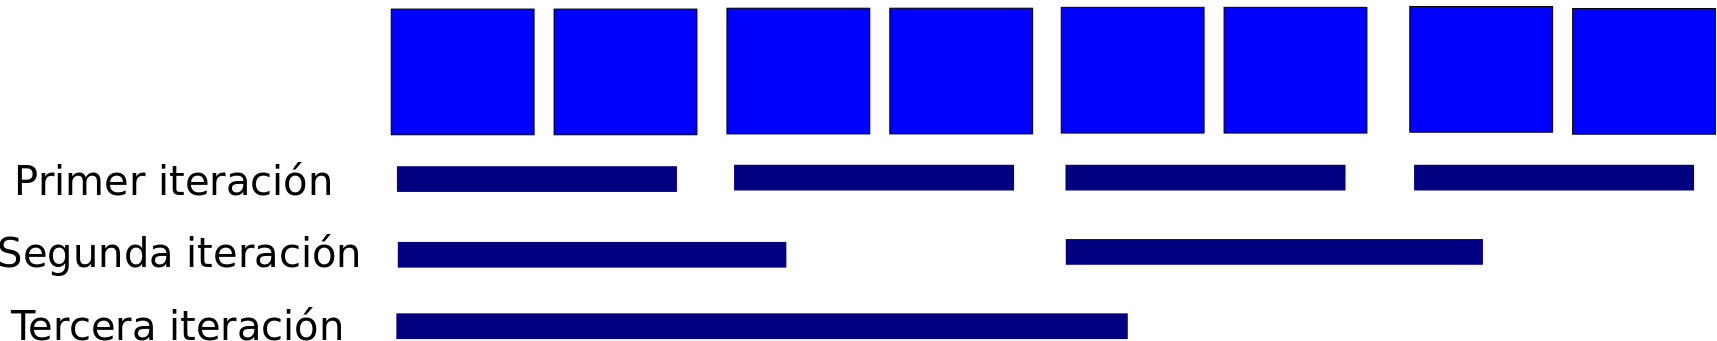
\includegraphics[width=\plotwidth]{images/reductions.png}
   \caption{Esquema de las reducciones realizadas en cada iteraci\'on del ciclo de la
   figura~\ref{code:sum-matrix-bench-code}.}
   \label{fig:sum-matrix-bench-reduce}
\end{figure}

Claramente este algoritmo debiera producir un mejor tiempo de ejecuci\'on, en
teor\'ia, utilizando m\'ultiples procesadores. Los c\'alculos son independientes
entre si y no se necesita ninguna sincronizaci\'on o datos comunes (caracter\'istica
denominada \textit{embarrasingly parallel} en la jerga).

Medimos los tiempos de reducir $128$ matrices de $1024 \times 1024$ elementos de punto
flotante de precisi\'on simple, variando la cantidad de hilos de ejecuci\'on a
utilizar. Para compensar por primeras lecturas y otros factores, se tomo un promedio
de los resultados despu\'es de realizar 20 mediciones sucesivas con la misma
cantidad de \textit{threads}. Todo el c\'odigo se incluye en un ap\'endice de este
trabajo.

Como puede verse en la figura~\ref{fig:sum-matrix-bench-result}, los resultados
son desalentadores: el uso de multiprocesamiento no es \'util para este problema,
a partir del uso de dos procesadores.

\begin{figure}[htbp]
   \centering
   \includegraphics[width=\plotwidth]{plots/cpu/scalability-matrix-sums.png}
   \caption{Tiempo en segundos para sumar 128 matrices de $1024 \times 1024$
   elementos, seg\'un la cantidad de threads usados. Los resultados corresponden
   a un promedio de 20 corridas, consecutivas para cada cantidad.}
   \label{fig:sum-matrix-bench-result}
\end{figure}

Observando el problema en si, notamos lo siguiente: Cada elemento de las
matrices a sumar es accedido de memoria una \'unica vez y el \'unico computo
realizado con este elemento es una suma con los dem\'as. La relaci\'on entre
lecturas de memoria y operaciones con los datos le\'idos es por lo tanto muy baja.

Observemos adem\'as que, al no utilizarse los datos m\'ultiples veces, cada l\'inea
de datos tiene un \textit{cache miss} asociado (el de la l\'inea donde reside) que
no se ve compensado por m\'as de un uso del dato mientras reside en cach\'e.

Este tipo de problemas se denomina \textit{memory bound}, ya que la velocidad del
\textit{bus} de memoria y la organizaci\'on de la misma es el factor determinante,
no la capacidad de computo o el tama\~no de los caches.

Esto implica que, pasado un cierto punto de velocidad de reloj de procesador y
cantidad de n\'ucleos, incrementar estos no produce mejoras apreciables. Esto es
lo que se puede ver en la figura~\ref{fig:sum-matrix-bench-result}. Es m\'as, el
\textit{overhead} de introducir nuevos hilos de ejecuci\'on incrementa el tiempo
de ejecuci\'on.

Ver que ese es el caso en la prueba de concepto realizada requiere herramientas
de an\'alisis m\'as sofisticadas. En nuestro caso utilizamos la herramienta de
c\'odigo abierto \textit{perf}. Este programa usa contadores de
\textit{performance} del procesador, que permiten llevar la cuenta de eventos de procesador
importantes como \textit{cache-misses} o \textit{stalls} de procesador, para dar estad\'isticas
a nivel arquitectural de la aplicaci\'on y de muy fino detalle.

A continuaci\'on se muestran los resultados de correr
un an\'alisis de \textit{perf} para 1 y 12 hilos simult\'aneos en la m\'aquina de
prueba. De inter\'es es el valor de \texttt{stalled-cycles-frontend}. Este valor
corresponde al contador de \textit{performance} \texttt{UOPS\_ISSUED.ANY}. Este
contador registra los eventos en los que el procesador esta \textit{stalleado},
es decir el \textit{pipeline } no avanza pues esta a la espera de datos que
lleguen de memoria principal~\cite{Intel3B}. En este
caso, parece ser que este factor es un limitante extremadamente fuerte.

{\footnotesize
\begin{verbatim}
$ perf stat -B ./benchmark 1024 128 1
1 0.180418953613844

 Performance counter stats for './benchmark 1024 128 1':

       2076,031257 task-clock                #    0,998 CPUs utilized
               225 context-switches          #    0,108 K/sec
                 0 cpu-migrations            #    0,000 K/sec
            67.583 page-faults               #    0,033 M/sec
     4.325.757.818 cycles                    #    2,084 GHz
     3.685.447.979 stalled-cycles-frontend   #   85,20% frontend cycles idle
   <not supported> stalled-cycles-backend
     1.801.562.845 instructions              #    0,42  insns per cycle
                                             #    2,05  stalled cycles per insn
       220.639.658 branches                  #  106,280 M/sec
           191.368 branch-misses             #    0,09% of all branches

       2,080571933 seconds time elapsed

$ perf stat -B ./benchmark 1024 128 12
12 0.182727314613294

 Performance counter stats for './benchmark 1024 128 12':

      22160,476291 task-clock                #   10,531 CPUs utilized
             2.402 context-switches          #    0,108 K/sec
                17 cpu-migrations            #    0,001 K/sec
            66.704 page-faults               #    0,003 M/sec
    46.310.011.626 cycles                    #    2,090 GHz
    42.797.073.792 stalled-cycles-frontend   #   92,41% frontend cycles idle
   <not supported> stalled-cycles-backend
     9.369.677.336 instructions              #    0,20  insns per cycle
                                             #    4,57  stalled cycles per insn
     2.657.329.767 branches                  #  119,913 M/sec
           687.016 branch-misses             #    0,03% of all branches

       2,104317579 seconds time elapsed
\end{verbatim}
}

Esto lleva a concluir que esta operaci\'on final impactar\'ia muy
negativamente en la escalabilidad de la implementaci\'on, y que por lo tanto a
medida que la cantidad de procesadores se incrementara esta secci\'on del
c\'odigo se har\'ia mucho m\'as pesada. Por lo tanto, se busc\'o reorganizar
este ciclo para no necesitar una matriz separada para cada \textit{thread}.

El ciclo a modificar esta en la figura~\ref{algo:rmm-output-previous}.
Se ve f\'acilmente que esto es posible si se invierten los ciclos internos y externos en
el algoritmo, para poder dividir los \'indices de la matriz global entre m\'ultiples
hilos de ejecuci\'on.

\begin{algorithm}[H]
    \centering
    \caption{C\'alculo original de la matriz de Kohn-Sham}
    \label{algo:rmm-output-previous}
    \begin{algorithmic}
        \State $R \gets 0_{m,n}$
        \State $F \gets functiones(PG)$
        \ForAll{$p \in puntos(PG)$}
            \ForAll{$i,j \in m \times n$}
            \State $R_{i,j} \gets R_{i,j} + F_{p,i} \cdot F_{p,j} \cdot factores_{p}$
            \EndFor
        \EndFor
        \ForAll{$i,j \in indices\_kohn\_sham(PG)$}
            \State $KS_{i,j} \gets KS_{i,j} + R_{i,j}$
        \EndFor
    \end{algorithmic}
\end{algorithm}

La versi\'on modificada puede verse en la figura~\ref{algo:rmm-output-new}. Lo que
se hace para este caso es recorrer los \'indices a actualizar de la matriz total
y para cada \'indice obtener la contribuci\'on de todos los puntos. Dado que cada \'indice debe
ser actualizado por, a lo sumo, un solo hilo de ejecuci\'on, no hay necesidad de
clonar matrices y reducirlas.

\begin{algorithm}[H]
    \centering
    \caption{C\'alculo de la matriz de Kohn-Sham reestructurado para paralelismo}
    \label{algo:rmm-output-new}
    \begin{algorithmic}
        \State $R \gets 0_{m,n}$
        \State $F \gets functions(PG)^T$
        \ForAll{$i,j \in indexes$}
            \State $KS_{i,j} \gets KS_{i,j} + \displaystyle \Sigma_{p \in points(PG)} F_{p,i} \cdot F_{p,j} \cdot factors_{p}$
        \EndFor
    \end{algorithmic}
\end{algorithm}

Un problema provocado por la implementaci\'on es que recorre la matriz de funciones
en orden de columnas, en lugar de orden por filas. Este orden es poco amigable
para los caches ya que cada fila de la matriz probablemente resida en l\'ineas de
cach\'e diferentes. Esto puede disminuir apreciablemente la performance del algoritmo.
Adem\'as, lastima su escalabilidad en procesadores, al incrementarse la cantidad de
invalidaciones de cach\'e y por lo tanto el \textit{overhead} del algoritmo de
coherencia de caches intreprocesadores.

La soluci\'on a este problema es sin embargo sencilla, trasponiendo la matriz de
valores de funciones. La misma puede trasponerse una vez y almacenarse en memoria
RAM al iniciar las iteraciones, teniendo por lo tanto un relativo bajo costo de
creaci\'on. Ahora entonces el orden de iteraci\'on de la misma es por filas, el
cual es \textit{cache-friendly}.

Esta modificaci\'on del algoritmo introduce un nuevo aspecto a considerar, similar
a las consideraciones hechas para la cantidad de puntos y funciones: una poca
cantidad de \'indices a actualizar en un mismo grupo eclipsa el \textit{overhead}
que introduce el uso de OpenMP. La cantidad de \'indices de la matriz de Kohn-Sham a
actualizar tambi\'en tiene una distribuci\'on bastante dispar, como puede verse
para el caso de ejemplo de hemoglobina en la figura~\ref{fig:histogram-indexes-hemo}.

\begin{figure}[htbp]
   \centering
   \includegraphics[width=\plotwidth]{plots/cpu/histogram-indexes-hemo.png}
   \caption{Cantidad de \'indices a actualizar de la matriz de Kohn-Sham}
   \label{fig:histogram-indexes-hemo}
\end{figure}

Esto enfatiza a\'un m\'as la necesidad de utilizar una paralelizaci\'on h\'ibrida
para grupos chicos y grandes, ya que ahora se tiene un factor m\'as que determina
cuanto trabajo se le asigna a los \textit{threads}.

Estos dos factores se tienen en cuenta en la funci\'on que determina si un grupo
es considerado grande o no. Para considerar un grupo grande, el mismo debe tener
una cantidad de puntos y una cantidad de \'indices en la matriz de Kohn-Sham mayor que
un valor de frontera (\textit{threshold}) multiplicado por la cantidad de hilos de
ejecuci\'on a realizar.

\subsection{Algoritmo de segregaci\'on}

Ya paralelizados los ciclos internos y armada la partici\'on,  tenemos que determinar
cuando un grupo es grande y chico, para
decidir si lo agregamos a alguna carga para un procesador. Como lo que
queremos es evitar resolver un grupo con insuficiente cantidad de puntos y/o
funciones en relaci\'on a la cantidad de n\'ucleos del sistema, usamos un
proceso de decisi\'on sencillo: si el grupo tiene m\'as puntos e \'indices a
actualizar que un cierto \textit{threshold} multiplicado por la cantidad de
\textit{threads} a utilizar, lo consideramos grande, sino lo consideramos chico.

Con esto lo que queremos conseguir es que cada \textit{thread} este ocupado una
cantidad de tiempo lo mayor posible: menos trabajo para cada procesador implica
que los \textit{overheads} de sincronizaci\'on se hacen m\'as notorios. Para eso,
sabiendo que la cantidad de trabajo depende de la cantidad de puntos e \'indices
de la matriz de Kohn Sham, queremos que cada thread sea asignado una cantidad de
inter\'es de estos.

Para decidir el valor de \textit{threshold} probamos con diversos valores para
el caso de la hemoglobina. De los valores resultantes mostramos algunos de los
resultados en la figura~\ref{fig:split-hemo}. En base a estos resultados decidimos
un valor de \textit{threshold} de 80 para nuestras pruebas posteriores.

Si bien parece que la diferencia es de poca importancia, es importante se\~nalar
que, siendo que apuntamos a lograr la mayor escalabilidad posible, diferencias
peque\~nas importan en el \textit{speedup} obtenido.

\begin{figure}[htbp]
   \centering
   \includegraphics[width=\plotwidth]{plots/cpu/different-splits.png}
   \caption{Valor del tiempo de iteraci\'on de XC en milisegundos, para distintos
   valores del \textit{threshold} de cantidad de puntos y matriz de Kohn Sham
   a asignar a cada \textit{thread}}
   \label{fig:split-hemo}
\end{figure}

\subsection{Algoritmo de balanceo}

Por \'ultimo, si bien el algoritmo de particionado y la funci\'on de costo son
buenas para los casos estudiados, no son perfectas. Como puede verse en la
figura~\ref{fig:lio-imbalance-between-loads}, hay una diferencia entre cargas
no despreciable en algunos casos, con lo cual todav\'ia se puede obtener algo de
mejoras en \textit{performance} entre iteraciones utilizando balanceo de cargas,
que obtuvo buenos resultados en la implementaci\'on para GPGPUS.

\begin{figure}[htbp]
   \centering
   \begin{subfigure}[b]{\plotwidthtres}
     \includegraphics[width=\textwidth]{plots/cpu/group-split-differences.png}
     \caption{Previo al balance.}
     \label{fig:lio-imbalance-between-loads}
   \end{subfigure}
   \begin{subfigure}[b]{\plotwidthtres}
     \includegraphics[width=\textwidth]{plots/cpu/group-split-differences-post-balance.png}
     \caption{Posterior al balance.}
     \label{fig:lio-imbalance-fixed}
   \end{subfigure}
   \caption{Comparaci\'on de los tiempos de ejecuci\'on para las distintas
   cargas asignadas a cada hilo de ejecuci\'on en el caso de la hemoglobina.}
   \label{fig:lio-imbalance}
\end{figure}

El algoritmo es muy similar, se mide el tiempo de \textit{runtime} para cada
grupo de cada carga, y cuanto dura cada una de ellas. Luego, se repite una
cantidad de veces (5 veces, como la implementaci\'on de balanceo en multiplaca)
que se mueve una cierta cantidad de grupos desde la carga m\'as pesada a la
m\'as liviana, de manera de no pasarse de la diferencia temporal que hay entre
ellas. Una vez movidos los grupos correspondientes, y tal que la diferencia
entre los dos estimativos es menor que el 5\% del peso total de la carga m\'as
pesada, se prosigue por encontrar las otras dos cargas m\'as dispares y
rebalancearlas. Para m\'as detalles del algoritmo puede verse la secci\'on
de balanceo de cargas de la implementaci\'on en GPU.

El costo computacional ya se vio anteriormente que resulta bajo. En el caso
de la hemoglobina se consigue menos del 5\% de diferencia en una iteraci\'on
de rebalanceo, obteni\'endose los resultados de la figura~\ref{fig:lio-imbalance-fixed}.

\subsection{Resultados preliminares}

Considerando la paralelizaci\'on del c\'odigo utilizamos el ejemplo de la
hemoglobina como base. En la figura~\ref{fig:hemo-scale} se puede ver la
escalabilidad conseguida en tiempo de ejecuci\'on con 12 procesadores.

\begin{figure}[htbp]
   \centering
   \includegraphics[width=\plotwidthsmaller]{plots/cpu/post-paralelizar-iteracion.png}
   \caption{Tiempo en milisegundos para la iteraci\'on del c\'alculo de la energ\'ia
   XC para la hemoglobina en la m\'aquina de prueba, seg\'un cantidad de \textit{threads}}
   \label{fig:hemo-scale}
\end{figure}

El resultado corresponde a un \textit{speedup} de 11,35 veces. De acuerdo
a la ley de Amdahl esto implica que 99.4\% de la iteraci\'on fue efectivamente
paralelizada, lo cual implica que la escalabilidad lograda en la m\'aquina de
prueba para este caso es muy cercana a la m\'axima.

Otro aspecto de inter\'es es que, posteriormente de hacer todos los cambios
necesario para lograr que el c\'odigo sea paralelizado, incluso la performance
en un solo procesador mejor\'o con respecto a lo original, para el caso de ejemplo,
como puede verse en la figura~\ref{fig:post-paralelizacion-single}.

No hay una optimizaci\'on \'unica que haya llevado a este cambio, pero la
reestructuraci\'on mejor\'o el uso de las matrices (muchas no necesitan ser
llenadas con ceros previo la iteraci\'on ni creadas todas las iteraciones) y
adem\'as se removieron algunas operaciones redundantes: los factores se calculan
una \'unica vez, los \'indices a calcular para cada grupo se mantienen entre
iteraciones disminuyendo la cantidad de c\'omputos a realizar, etc.

Ninguna de estas optimizaciones en si aporta demasiado pero la combinaci\'on
da una mejora no despreciable.

\begin{figure}[htbp]
   \centering
   \includegraphics[width=\plotwidthsmaller]{plots/cpu/post-paralelizar-iteracion-single.png}
   \caption{Tiempo en milisegundos para la iteraci\'on del c\'alculo de la energ\'ia
   XC para la hemoglobina en la m\'aquina de prueba, para la versi\'on
   post paralelizaci\'on en un solo procesador}
   \label{fig:post-paralelizacion-single}
\end{figure}

\subsection{Paralelizaci\'on a funciones y pesos}

Aunque nos concentramos en mejorar la iteraci\'on del c\'omputo de la energ\'ia
de intercambio y correlaci\'on, porque es la parte m\'as pesada y la misma se
ejecuta muchas veces (51 en el caso de la hemoglobina), realizamos unas mejoras
al c\'alculo de los pesos de cada punto de la grilla, y al c\'omputo de
las funciones por grupo. Estos cambios son detallados en esta secci\'on.

En el caso del c\'alculo de pesos por grupo, esto resulto ser sencillo: el
c\'omputo consiste de un \'unico ciclo sobre todos los puntos, y luego filtrar los
puntos que sean despreciables. Separando este ciclo en dos, pudimos f\'acilmente
paralelizar el primero con OpenMP de manera an\'aloga a los anteriores.

Los resultados son buenos, aunque no demasiado: el ciclo escala 10 veces con 12
\textit{threads} para el caso de la hemoglobina, como puede verse en la figura
~\ref{fig:weights-paralelizado}. El ciclo de filtrado de puntos no es f\'acilmente
paralelizable puesto que se deben agregar los elementos en orden a un arreglo
de grupos.

\begin{figure}[htbp]
   \centering
   \includegraphics[width=\plotwidthsmaller]{plots/cpu/post-paralelizar-pesos.png}
   \caption{Tiempo en milisegundos para la paralelizaci\'on del c\'omputo de los pesos
    de la grilla de integraci\'on, seg\'un cantidad de \textit{threads}}
   \label{fig:weights-paralelizado}
\end{figure}

El caso de funciones es m\'as interesante, porque los resultados obtenidos son
bastante malos: Si bien calcular las funciones para cada grupo es una tarea muy
paralelizable en teor\'ia,porque son completamente independientes, a diferencia de
los c\'alculos de la iteraci\'on, estos no han sido los resultados obtenidos.

Por un lado, empezamos por evitar las proyecciones de matrices realizando todos
los c\'alculos usando las matrices de componentes. Esto aumento la performance de
manera significativa, como puede verse en la figura~\ref{fig:lio-post-elim-proy}.
Esto se condice con los resultados que obtuvimos para la iteraci\'on tambi\'en.

\begin{figure}[htbp]
   \centering
   \includegraphics[width=\plotwidthsmaller]{plots/cpu/post-mejorar-functions-single-core.png}
   \caption{Tiempo en milisegundos del c\'omputo de todas las matrices para todos
   los grupos en el caso de la hemoglobina, antes y despu\'es de usar las matrices por
   componente.}
   \label{fig:lio-post-elim-proy}
\end{figure}

La causa nuevamente es una baja relaci\'on entre c\'omputo y accesos a memoria,
y la disparidad de costo entre grupos. La primera dificulta la divisi\'on de los
puntos del grupo entre hilos de ejecuci\'on, mucho m\'as que en el caso de la iteraci\'on: en la iteraci\'on los
valores de las matrices eran reutilizados. La segunda dificulta, al igual que antes, la
paralelizaci\'on externa, en la que subconjuntos de los grupos son resueltos
en paralelo por \textit{threads} distintos.

Para tratar de paliar este efecto en la paralelizaci\'on externa, utilizamos un
\textit{scheduler} guiado, donde cada \textit{thread} va recibiendo porciones
fijas de las iteraciones de manera din\'amica. De esta manera un \textit{thread}
muy cargado recibir\'a menos iteraciones mientras que los ociosos reciben otras.

El funcionamiento de esta estrategia no esta asegurado puesto que el \textit{runtime}
de OpenMP no tiene conocimiento \textit{a priori} de los costos, como si lo tenemos
nosotros en el caso de la divisi\'on de la iteraci\'on por ejemplo.

Los resultados pueden verse en la figura~\ref{fig:functions-paralelizado}. La
paralelizaci\'on externa es mejor que la interna, pero ambas escalan mal (menos
de un 6x) para 12 procesadores. Aunque la importancia no es tanta para estos
c\'alculos porque se realizan una vez, sirven tambi\'en de punto de comparaci\'on
con el trabajo realizado para paralelizar la iteraci\'on.

\begin{figure}[htbp]
   \centering
   \includegraphics[width=\plotwidthsmaller]{plots/cpu/post-paralelizar-functions.png}
   \caption{Tiempo en milisegundos para la paralelizaci\'on del c\'omputo
   de matrices para los grupos, seg\'un tipo de paralelizaci\'on y cantidad de
   \textit{threads}}
   \label{fig:functions-paralelizado}
\end{figure}
